\documentclass[10pt,twocolumn,letterpaper,french]{article}

\usepackage[utf8]{inputenc} 

\usepackage{cvpr}
\usepackage{times}
\usepackage{epsfig}
\usepackage{graphicx}
\usepackage{amsmath}
\usepackage{amssymb}
\usepackage[francais]{babel}


\pagenumbering{gobble}

% Include other packages here, before hyperref.

% If you comment hyperref and then uncomment it, you should delete
% egpaper.aux before re-running latex.  (Or just hit 'q' on the first latex
% run, let it finish, and you should be clear).
\usepackage[breaklinks=true,bookmarks=false]{hyperref}

\cvprfinalcopy % *** Uncomment this line for the final submission

\def\cvprPaperID{****} % *** Enter the CVPR Paper ID here
\def\httilde{\mbox{\tt\raisebox{-.5ex}{\symbol{126}}}}

% Pages are numbered in submission mode, and unnumbered in camera-ready
%\ifcvprfinal\pagestyle{empty}\fi
\setcounter{page}{4321}
\begin{document}

%%%%%%%%% TITLE
\title{Transfert d'apprentissage pour le suivi d'objets\\par réseaux siamois}

\author{Paulin Brissonneau\\
CentraleSupélec\\
{\tt\small paulin.brissonneau@student-cs.fr}}
% For a paper whose authors are all at the same institution,
% omit the following lines up until the closing ``}''.
% Additional authors and addresses can be added with ``\and'',
% just like the second author.
% To save space, use either the email address or home page, not both



\maketitle
%\thispagestyle{empty}

%%%%%%%%% ABSTRACT
\begin{abstract}

Les avancées récentes en suivi d'objet tirent leur profit de métriques de similitude approximées par des réseaux de neurones profonds. Le temps d'inférence de telles méthodes, qui se doivent de fonctionner en temps réel, a été diminué par des architectures de type réseaux siamois, au prix d'un apprentissage \textit{offline} très coûteux en calculs. Dans ce rapport, nous nous intéressons à la possibilité d'utiliser des réseaux pré-entraînés pour obtenir des réseaux extracteurs de caractéristiques de qualité en un temps d'apprentissage \textit{offline} minimal. Nous montrons qu'il est possible de s'appuyer sur des réseaux pré-entraînés même sur des problèmes différents (classification et segmentation). Nous proposons une méthode générale pour diminuer efficacement le temps d’entraînement en gardant des performances correctes.
 
\end{abstract}

%%%%%%%%% BODY TEXT
\section*{Introduction}

Le suivi d'objets est un domaine de la vision numérique qui consiste à suivre un ou plusieurs objets présents sur une vidéo.
   Pendant longtemps, l'état de l'art était tenu par des algorithmes purement statistiques, qui associaient des probabilité de correspondance entre les formes présentes sur deux images à la suite dans une vidéo. C'est le cas par exemple des méthodes [REF], qui proposent des performances encore respectables pour certains problèmes.
   Depuis quelques années, le domaine du suivi d'objets a été drastiquement influencé par le développement de l'apprentissage profond. En quelques années, les algorithmes basés sur des métriques profondes ont détrôné tous les algorithmes classiques à l'état de l'art. L'utilisation de réseaux profonds permet une comparaison plus fine des différents objets et résiste mieux aux occlusions de longue durée. \\
   
   L'introduction des réseaux profonds en suivi d'objets prend plusieurs formes. Les méthodes basées sur les détections infèrent le suivi en deux étapes distinctes : d'abord une détection d'objets présents sur l'image, puis une association des différents objets d'une image à la suivante. Cette façon de faire donne des résultats remarquables pour un temps de calcul des inférence court. Les algorithmes SORT [REF]  sont des représentants de cette famille. Un avantage considérable à séparer les deux étages (détection et suivi) réside dans le fait de pouvoir réutiliser des algorithmes de détection déjà existants. Il est par exemple habituel de baser ces approches sur un YOLO ou un RCNN. Cela permet de transférer l'apprentissage à partir du problème très classique de détection vers le problème de suivi, le transfert d'apprentissage est pour ainsi dire quasi-direct. [REF] ont proposé (deepSORT [REF]) d'ajouter une métrique profonde de similarité des objets dans le deuxième étage (suivi). Cette métrique est approximée par un réseau de neurone profond. \\
   
   Comme l'on fait remarquer [REF], les méthodes à deux étages ont une limitation intrinsèque : l'indépendance des deux étages provoque une redite des calculs d'extraction de caractéristiques. Les premières couches du premier étage qui se charge de la détection, ont un rôle très proche des couches du deuxième étage qui calcula la métrique se similarité. De nombreux travaux ont tenté d'unifier ces deux étages avec différentes méthodes. Par exemple, [REF] [REF] [REF]. L'unification de la méthode a pour effet de réduire fortement le temps de calcul nécessaire à l'inférence, mais cela se fait au prix d'un entraînement \textit{offline} très long qui découle l'impossibilité d'utiliser des réseaux détecteurs pré-entraînés.\\
   
   Parmi les solutions unifiées, celles basées sur les réseaux siamois se sont emparées de l'état de l'art et montrent des performances très prometteuses. La limitation principale cette méthode réside dans le fait qu'il est impossible d'utiliser des extracteurs ou détecteurs classiques. L'apprentissage \textit{offline} est très coûteux en temps de calcul et nécessite des ensemble de données conséquents et spécialisés, souvent inaccessibles suivant la nature du problème et les moyens disponibles pour entraîner l'algorithme. C'est pourquoi il est intéressant de se demander dans quelle mesure le transfert d'apprentissage est efficace pour les réseaux siamois, ainsi que de déterminer de quels problèmes classiques (classification ou segmentation) il est pertinent d'utiliser les pré-entraînements. (dire que SiamMask : proches) \\
   
  Nous étudions exclusivement le transfert d'apprentissage et ne cherchons pas à atteindre les performances de l'état de l'art. C'est pour cette raison que nous utiliserons l'architecture simple du siamFC [REF], et non des architectures plus récentes et plus poussées qui présentent de meilleurs résultats. Grâce à une architecture de référence sobre, nous seront plus à même d'étudier en détail l'effet transfert d'apprentissage et d'interpréter nos résultats sans autres effets parasites que pourraient apporter des architectures complexes.
  
(désengorger l'intro pour mettre plus de masse dans l'état de l'art)
   

\section*{État de l'art}

\subsubsection*{Réseaux Siamois}

Les réseaux siamois sont une ancienne idée qui a fait son apparition en 1994 grâce à Bromley et al. \cite{siamese}. Le principe des réseaux siamois est d'encoder de manière non-linéaire deux entrées différentes avec un même réseau extracteur de caractéristiques. L'objectif est que les cartes de caractéristiques obtenues soient porteuses de suffisamment d'information sémantique pour pouvoir comparer les données initialement données en entrée. À titre d'exemple, pour comparer deux visages et dire si ils appartiennent à la même personne, on encode chacun des deux visages par un seul et même réseaux, la comparaison des cartes de caractéristiques nous donnera une idée de la similarité des deux visages, non pas d'un point de vu photographique, mais d'un point de vue sémantique. \\

Les réseaux siamois sont donc constitués de principalement deux étages, plus ou moins séparés selon les applications. La structure globale d'un réseau siamois est explicité sur la figure \ref{siamese}. Le première étage est l'extracteur de caractéristiques, lorsque les données sont structurées et compositionnelles il s'agira le plus souvent d'un réseau convolutionnel. Le deuxième étage permet la comparaison des caractéristiques extraites peut prendre plusieurs formes différentes, allant de la simple distance vectorielle au réseau de neurone. Il y a parfois un étage intermédiaire permettant de fusionner les cartes de caractéristiques. Il peut s'agir par exemple d'une simple soustraction terme à terme ou d'une corrélation croisée (\textit{cross-correlation}).\\

\begin{figure}[!h]
\centering
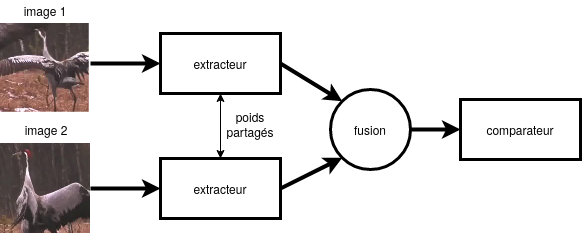
\includegraphics[width=240pt]{images/siamese.png} 
\caption{Structure générale des réseaux siamois.}
\label{siamese}
\end{figure}

Les réseaux siamois ont été utilisés pour un très grand nombre de tâches, à savoir le \textit{hashing} \cite{hashing}, le \textit{clustering} \cite{clustering} et surtout l'apprentissage sur peu d'exemples (\textit{few-shot learning}) \cite{one-shot}. De par leur structure, ils sont aussi particulièrement adapté à la comparaison de deux données, comme par exemple la vérification faciale \cite{face_verif}, la localisation \cite{tompson2015efficient}, la rénovation d'images \cite{gordo2017endtoend}, et bien sûr le suivi d'objets \cite{siamfc, siamfcplusplus, siamMask, trackRCNN}.

\subsubsection*{Suivi d'objets}

\subparagraph{a. Approches classiques\\\\} 

Les premières approches pour le suivi \textit{online} étaient basées sur des filtres de Kalman \cite{Kalman}. C'est un filtre récursif bayésien dont l'objectif est de calculer une distribution de probabilité pour la position de l'objet d'une image à la suivante dans la vidéo. Le filtre couple les informations venant de l'observation supposée altérée par un bruit gaussien, et celles venant d'un modèle dynamique de l'objet qui prend typiquement la forme d'un modèle de vitesse constante pour chaque objet de l'image. Une autre méthode classique est le filtre à particules, qui approxime la distribution de probabilité de présence par la densité d'un groupe de particules \cite{particule}. \\

Ces méthodes sont adaptées pour le suivi d'un seul objet sur une image (problème \textbf{SOT} pour \textit{Single Object Tracking}) , cependant pour suivre plusieurs objets il faut ajouter une méthode d'association de chaque objet à l'image suivante. Le problème de suivi simultané de plusieurs objets est appelé \textbf{MOT} (pour \textit{Multiple Object Tracking}). Les deux méthodes historiques pour le problème MOT sont \textbf{MHT} (\textit{Multi-Hypothesis Tracker}) et \textbf{JPDA} (\textit{Joint Probabilistic Data Association}).

Les méthodes \textbf{MHT} \cite{chenouardMHT, MHTrevisited} considèrent et stockent en mémoire toutes les associations possibles entre tous les objets de chaque image et ceux de l'image suivante. Chaque probabilité d'associations est raffinées en se basant sur les images suivantes. L'attente des images suivantes permet d'appréhender efficacement les occlusions puisque l'on peut attendre que l'objet réapparaisse. Cela apporte aussi son lot d'inconvénients, notamment, le suivi \textit{online} est impossible, et le coût calculatoire d'un tel algorithme est considérable.

Les méthodes \textbf{JPDA}, \cite{FortmannJPDA, JPDArevisited} sont des méthodes purement statistiques. À chaque image, l'algorithme liste tous les candidats possibles selon une fenêtre de positions jugées acceptables. La probabilité a posteriori de chaque candidat est calculée, en considérant que les autres candidats sont des erreurs distribués selon une loi de Poisson. Encore une fois, le coût calculatoire de cet algorithme est considérable et ne permet pas de l'appliquer à beaucoup de problèmes concrets.

Bien que ces méthodes en elle-même soient dépassées, elles importantes à mentionner car comme on va le voir certaines méthodes plus modernes leur font écho et les problèmes de coûts calculatoires dont elles souffrent sont, eux, toujours d'actualité.

\subparagraph{b. Approches modernes\\\\} 

L'utilisation des réseaux de neurones pour le suivi d'objet annonce beaucoup d'avantages. Notamment cela permet de s'appuyer sur des métriques de similarité plus pertinentes entre les différents objets. Alors que les méthodes classiques se contentaient d'utiliser des modèles de mouvement et d'apparence superficielle, les métriques profondes peuvent reconnaître des objets malgré des occlusions très longues, même dans le cas où l'apparence de l'objet a changé (un objet dont le point de vue a changé par exemple).

Une première façon de mettre à profit les réseaux de neurones pour le suivi a été de développer des méthodes à deux étages : d'abord une détection d'objets présents sur l'image, puis une association des différents objets d'une image à la suivante. C'est ce qu'ont proposé Bewley et al. \cite{SORT} avec l'algorithme \textbf{SORT}. Il repose sur l'idée très simple d'utiliser les détections d'un détecteur classique (YOLO ou RCNN par exemple) pour ensuite appliquer un filtre de Kalman qui se chargera d'associer les différents objets d'une frame à la suivante. Il s'inspire donc directement des méthodes classiques du pragraphe précédent. Le filtre de Kalman impose intrinsèquement une hypothèse de vitesse constante pour chacun des objets détecter, on comprend donc que cette méthode est limitée lorsque les objets détectés font des mouvements brusques comme c'est le cas quand la caméra bouge. Pour remédier à ce problème, Wojke et al. \cite{deepSORT} ont proposé de coupler le SORT à une métrique profonde spécialement conçue pour comparer les apparences de deux objets. Cette petite modification permet de raffiner la méthode d'association du SORT et d'associer des objets plus éloignés dans le temps et dans l'espace. DeepSORT donne des résultats remarquablement proches de l'état de l'art pour un coût calculatoire faible plus faible que toutes les autres méthodes.

Les méthodes à deux étages ont une limitation intrinsèque : l'indépendance des deux étages provoque une redite des calculs d'extraction de caractéristiques. Les premières couches du premier étage qui se charge de la détection, ont un rôle très proche des couches du deuxième étage qui calcula la métrique se similarité. Les travaux se sont donc centrés sur des méthodes unifiées, selon lesquelles un seul réseau doit pouvoir extraire un maximum d'informations et pouvoir résoudre le problème de détection puis de suivi en une seule inférence.

Étant donnée la nature récursive du problème, les études se sont concentrée sur l’entraînement de \textbf{réseaux récursif} (RNN). Gan et al. \cite{RNNtracking} ont proposé d'utiliser un RNN pour prédire directement la position de l'objet traqué dans l'image. Cette méthode a été ensuite améliorée par Ebrahimi-Kahou et al. \cite{RATM} par l'ajout de mécanisme d'attention pour donner le RATM (\textit{Recurrent Attentive Tracking Model}). \\

En faisant le constat que ces méthodes étaient prometteuses sans pour autant montrer des résultats à l'état de l'art, de nombreuses équipes ont proposé de remplacer les réseaux récurrents par des réseaux siamois, qui peuvent être assimilés à des réseaux récurrent manipulant des séquences de deux images. Il n'est pas possible d’entraîner à partir de zero un réseau pour chaque vidéo, il font donc s'appuyer sur un apprentissage \textit{offline} pour ensuite simplifier l'apprentissage \textit{online} qui se fera sur la vidéo elle-même. C'est ce qu'ont proposé Wang et al. avec SO-DLT \cite{wang2015transferring} et Nam et al. avec MDNet \cite{nam2016learning}, cependant cela oblige à continuer l'apprentissage même pendant le suivi \textit{online}, ce qui est coûteux en calcul et ne permet pas d'atteindre du temps-réel. D'autres travaux, comme Wang et al. avec le FCNT \cite{Wang} ou encore Held et al. \cite{held2016learning}, ont tenté de complètement se passer d'apprentissage \textit{online}, en se basant complètement sur les caractéristiques profondes extraites grâce à un réseau pré-entraîné complètement en \textit{offline}. Ces méthodes ne sont pas complètement convolutionnels, ce qui implique des réseaux toujours trop lourds pour des applications en temps réel, en plus de nécessité une augmentation importante des données pour forcer l'invariance à la translation. Bertinetto et al. \cite{siamfc} ont proposé siamFC, qui est un réseau siamois complètement convolutionnel (\textit{Fully-Convolutionnal Siamese network}). Le siamFC est le premier réseau à proposer une inférence (\textit{online}) en temps-réel tout en assurant des résultats remarquables. Cette méthode est le point de départ de nombreuses améliorations qui ont chacune leur tour donnée des résultats à l'état de l'art en SOT (\textit{Single Object Tracking}). En particulier  siamMask (2018) \cite{siamMask}  propose de coupler le suivi à une tâche de segmentation, siamFc++ (2020) \cite{siamfcplusplus}  entraîne un seule architecture unifiée à quatre tâches différentes : la classification, l'estimation du prochain état de l'objet, un suivi sans \textit{prior}, et une estimation globale de la qualité du suivi. Les résultats du siamFC++ sont aujourd'hui inégalés. Notons que les méthode à réseau siamois convolutifs donnent aussi des performances remarquables en MOT (\textit{Multiple Objet Tracking}), puisque le track-RCNN (2020)  \cite{trackRCNN}, qui est un réseau siamois aidé d'un extracteur de RoI (\textit{Region of Interest}) est actuellement l'algorithme le plus performant en MOT. Tous ces algorithmes infèrent (\textit{online}) le suivi d'objets plus rapidement que les standards du temps réels, au prix d'un apprentissage \textit{offline} très coûteux en terme de calculs.


\subparagraph{c. Métriques}

https://cvhci.anthropomatik.kit.edu/~stiefel/papers/ECCV2006WorkshopCameraReady.pdf

MANQUE DES REF

REF métrique de VOT : \cite{Kristan_2016}

Il existent différentes métriques pour mesurer les performances des modèles en suivi d'objets, elles ne sont pas out à fait les même si il s'agit d'une tâche SOT ou d'une tâche MOT. La métrique la plus classique est l'espérance du chevauchement moyen (\textit{expected average overlap}), où le chevauchement est l'indice de Jaccard (\textit{Intersection Over Union}). Cette métrique est aussi appelée la \textbf{précision du suiveur}. Cependant cette métrique ne permet pas d'avoir une bonne idée du comportement du suiveur, en effet deux modèles de même précision peuvent tout de même avoir un nombre différent d'échecs (c'est à dire de prédiction complètement fausses). La métrique qui permet de prendre en compte cet aspect de robustesse s'appelle le \textbf{taux de succès/échecs} (\textit{failures/succes rate}) ou encore appelée \textbf{robutesse du suiveur}. Il consiste à calculer la proportion de temps pendant lequel l'intersection de la prédiction et de la vérité étiquetée n'est pas nulle. Une combinaison de ces deux métriques peut donner une idée assez précise du comportement du modèle.
Dans ce rapport, nous nous intéressons à des modèles dont la particularité est de tourner en temps réel. Mesurer le nombre de \textbf{\textit{frame} par seconde (fps)} est donc important. La limite de valeur de nombre de fps pour considérer du temps réel n'est pas clairement définie mais une référence est la limite de 20 fps en vigueur dans le concours \textit {VOT real-time} \cite{VOT}.

Ces métriques sont tout de même simplistes et ne permettent pas toujours de comprendre tout la spécificité des comportement des suiveurs. Quelques projets ont eu pour objectif de normaliser les méthodes de mesure des performances de suivi. Notamment, Bernardin et al. \cite{metrics} ont proposé les métriques MOTP (\textit{Multiple Object Tracking Precision}) et MOTA (\textit{Multiple Object Tracking Accuracy}) qui prennent en compte tous les différents aspects des comportements des suiveurs. Cependant, jusqu'à maintenant, aucune mesure universelle ne fait l'unanimité. 

\section*{Approche}

\subsubsection*{Architecture}

Please follow the steps outlined below when submitting your manuscript to
the IEEE Computer Society Press.  This style guide now has several
important modifications (for example, you are no longer warned against the
use of sticky tape to attach your artwork to the paper), so all authors
should read this new version.

\subsubsection*{Ensemble de données}


Please follow the steps outlined below when submitting your manuscript to
the IEEE Computer Society Press.  This style guide now has several
important modifications (for example, you are no longer warned against the
use of sticky tape to attach your artwork to the paper), so all authors
should read this new version.

\subsubsection*{Métriques}

Please follow the steps outlined below when submitting your manuscript to
the IEEE Computer Society Press.  This style guide now has several
important modifications (for example, you are no longer warned against the
use of sticky tape to attach your artwork to the paper), so all authors
should read this new version.

\subsubsection*{Pré-entraînements}

Please follow the steps outlined below when submitting your manuscript to
the IEEE Computer Society Press.  This style guide now has several
important modifications (for example, you are no longer warned against the
use of sticky tape to attach your artwork to the paper), so all authors
should read this new version.

Tester sur : 
	- Type de dataset différent
	- Différents types de problèmes (segmentation, classification).
	- Un nouveau problème

\section*{Expérimentations}

Please follow the steps outlined below when submitting your manuscript to
the IEEE Computer Society Press.  This style guide now has several
important modifications (for example, you are no longer warned against the
use of sticky tape to attach your artwork to the paper), so all authors
should read this new version.

\subsubsection*{Détails d’entraînement}

Please follow the steps outlined below when submitting your manuscript to
the IEEE Computer Society Press.  This style guide now has several
important modifications (for example, you are no longer warned against the
use of sticky tape to attach your artwork to the paper), so all authors
should read this new version.

\section*{Conclusion}

Please follow the steps outlined below when submitting your manuscript to
the IEEE Computer Society Press.  This style guide now has several
important modifications (for example, you are no longer warned against the
use of sticky tape to attach your artwork to the paper), so all authors
should read this new version.




{\small
\bibliographystyle{ieee}
\bibliography{rapport}
}

\end{document}
